\documentclass[oneside,a4paper,14pt]{extarticle}
\usepackage[a4paper,letterpaper,top=20mm,bottom=20mm,left=20mm,right=10mm]{geometry}
\usepackage[russian]{babel}
\usepackage{indentfirst}
\usepackage{graphicx}
\usepackage{caption}
\usepackage{titlesec}
\usepackage{minted, fancyvrb}
\usepackage{hyperref}
\usepackage{enumitem}
\usepackage{amsmath}
\usepackage{fancyhdr}
\usepackage{colortbl}
\usepackage[dvipsnames]{xcolor}
\usepackage{tikz-timing}
\usepackage{tikz}
\usetikzlibrary{karnaugh}

% Настройка автоматических подписей к рисункам (Замена Рис. на Рисунок и тире в качестве разделителя)
\DeclareCaptionLabelSeparator{customdash}{~---~}
\captionsetup[figure]{name=Рисунок, labelsep=customdash, justification=centering}

% Форматирование листингов с кодом
\setminted{style = rainbow_dash, fontsize = \small} 

% Форматирование заголовков
\titleformat{\section}{\normalsize\bfseries}{\thesection}{1em}{}
\titleformat{\subsection}{\normalsize\bfseries}{\thesubsection}{1em}{}
\titleformat{\subsubsection}{\normalsize\bfseries}{\thesubsubsection}{1em}{}

% Интерлиньяж и абзац
\renewcommand\baselinestretch{1.33}
\setlength{\parindent}{1.25cm}  % длина красной строки

% Для всех списков
\setlist[enumerate]{
  left=0.5\parindent,    
  label=\arabic*.,       
  itemsep=0pt,           
  topsep=5pt,            
  partopsep=0pt,         
  parsep=0pt             
}

\setlist[itemize]{
  left=0.5\parindent,    
  itemsep=0pt,           
  topsep=5pt,            
  partopsep=0pt,
  parsep=0pt
}

% Гиперссылки
\hypersetup{
  colorlinks=true,
  linkcolor=black,
  urlcolor=blue,
  pdfborder={0 0 0},
  pdftitle={Синтез комбинационных схем в базисе И-НЕ: Дешифратор и Демультиплексор},
  pdfauthor={Черкасов А.А.},
}

\begin{document}

\newpage
\thispagestyle{empty}
\begin{center}
  МИНИСТЕРСТВО НАУКИ И ВЫСШЕГО ОБРАЗОВАНИЯ РОССИЙСКОЙ ФЕДЕРАЦИИ\\
  ФЕДЕРАЛЬНОЕ ГОСУДАРСТВЕННОЕ БЮДЖЕТНОЕ УЧРЕЖДЕНИЕ ВЫСШЕГО ОБРАЗОВАНИЯ\\
  <<ВЯТСКИЙ ГОСУДАРСТВЕННЫЙ УНИВЕРСИТЕТ>>\\
  Институт математики и информационных систем\\
  Факультет автоматики и вычислительной техники\\
  Кафедра электронных вычислительных машин
\end{center}
\vspace{10mm}

\hfill
\begin{tabular}{l}
  \footnotesize Дата сдачи на проверку:                                          \\
  \footnotesize <<\rule[-1mm]{5mm}{0.10mm}\/>>\rule[-1mm]{20mm}{0.10mm}\ 2026 г. \\
  \footnotesize Проверено:                                                       \\
  \footnotesize <<\rule[-1mm]{5mm}{0.10mm}\/>>\rule[-1mm]{20mm}{0.10mm}\ 2026 г. \\
\end{tabular}
\vfill

\begin{center}
  Отчёт по контрольной работе\\
  <<Синтез дешифратора и демультиплексора>>\\
  по дисциплине\\
  <<Цифровая схемотехника>>\\
\end{center}
\vspace{25mm}
\noindent
\begin{tabular}{ll}
  Разработал student гр. ИВТб-2301-05-00 & \hspace{20mm}\rule[-1mm]{30mm}{0.10mm}\,/Черкасов А.А./ \\
                                 & \hspace{27.5mm}\footnotesize(подпись)                   \\
  Преподаватель                  & \hspace{20mm}\rule[-1mm]{30mm}{0.10mm}\,/Мельцов В. Ю./  \\
                                 & \hspace{27.5mm}\footnotesize(подпись)                   \\
\end{tabular}

\noindent
\begin{tabular}{lp{58mm}r}
  Работа защищена &  & \hspace{8mm}<<\rule[-1mm]{8mm}{0.10mm}\/>>\rule[-1mm]{38mm}{0.10mm}\ 2026 г.
\end{tabular}
\vfill

\begin{center}
  Киров\\
  2026
\end{center}

\newpage\thispagestyle{plain}

\section{Цель работы}
Получить навыки синтеза многовыходных комбинационных логических устройств. Синтезировать функциональные схемы двоичного дешифратора <<4 в 16>> и демультиплексора <<1 в 16>> в функционально полном логическом базисе <<И-НЕ>> (базис Шеффера), изучить принципиальную взаимосвязь архитектур данных устройств.

\section{Условно Графическое Обозначение дешифратора}
\begin{figure}[H]
  \centering
  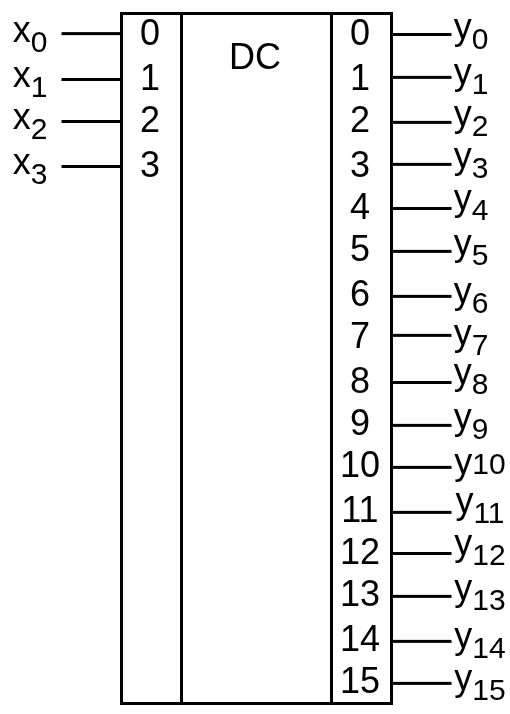
\includegraphics[width=0.85\textwidth,height=0.6\textheight,keepaspectratio]{pics/UGO.png}
  \caption{Условно-графическое обозначение дешифратора}
\end{figure}

\section{Таблица истинности дешифратора}
Двоичный дешифратор имеет 4 адресных входа ($x_3, x_2, x_1, x_0$) и 16 выходов ($y_0 \dots y_{15}$). Активным уровнем выходов является логическая единица.

\begin{center}
  Таблица 1 --- Таблица истинности дешифратора 4 в 16 \\
  \vspace{3mm}
  \resizebox{\textwidth}{!}{
    \begin{tabular}{cccc|cccccccccccccccc}
      $x_3$ & $x_2$ & $x_1$ & $x_0$ & $y_0$ & $y_1$ & $y_2$ & $y_3$ & $y_4$ & $y_5$ & $y_6$ & $y_7$ & $y_8$ & $y_9$ & $y_{10}$ & $y_{11}$ & $y_{12}$ & $y_{13}$ & $y_{14}$ & $y_{15}$ \\
      \hline
      0 & 0 & 0 & 0 & 1 & 0 & 0 & 0 & 0 & 0 & 0 & 0 & 0 & 0 & 0 & 0 & 0 & 0 & 0 & 0 \\
      0 & 0 & 0 & 1 & 0 & 1 & 0 & 0 & 0 & 0 & 0 & 0 & 0 & 0 & 0 & 0 & 0 & 0 & 0 & 0 \\
      0 & 0 & 1 & 0 & 0 & 0 & 1 & 0 & 0 & 0 & 0 & 0 & 0 & 0 & 0 & 0 & 0 & 0 & 0 & 0 \\
      0 & 0 & 1 & 1 & 0 & 0 & 0 & 1 & 0 & 0 & 0 & 0 & 0 & 0 & 0 & 0 & 0 & 0 & 0 & 0 \\
      0 & 1 & 0 & 0 & 0 & 0 & 0 & 0 & 1 & 0 & 0 & 0 & 0 & 0 & 0 & 0 & 0 & 0 & 0 & 0 \\
      0 & 1 & 0 & 1 & 0 & 0 & 0 & 0 & 0 & 1 & 0 & 0 & 0 & 0 & 0 & 0 & 0 & 0 & 0 & 0 \\
      0 & 1 & 1 & 0 & 0 & 0 & 0 & 0 & 0 & 0 & 1 & 0 & 0 & 0 & 0 & 0 & 0 & 0 & 0 & 0 \\
      0 & 1 & 1 & 1 & 0 & 0 & 0 & 0 & 0 & 0 & 0 & 1 & 0 & 0 & 0 & 0 & 0 & 0 & 0 & 0 \\
      1 & 0 & 0 & 0 & 0 & 0 & 0 & 0 & 0 & 0 & 0 & 0 & 1 & 0 & 0 & 0 & 0 & 0 & 0 & 0 \\
      1 & 0 & 0 & 1 & 0 & 0 & 0 & 0 & 0 & 0 & 0 & 0 & 0 & 1 & 0 & 0 & 0 & 0 & 0 & 0 \\
      1 & 0 & 1 & 0 & 0 & 0 & 0 & 0 & 0 & 0 & 0 & 0 & 0 & 0 & 1 & 0 & 0 & 0 & 0 & 0 \\
      1 & 0 & 1 & 1 & 0 & 0 & 0 & 0 & 0 & 0 & 0 & 0 & 0 & 0 & 0 & 1 & 0 & 0 & 0 & 0 \\
      1 & 1 & 0 & 0 & 0 & 0 & 0 & 0 & 0 & 0 & 0 & 0 & 0 & 0 & 0 & 0 & 1 & 0 & 0 & 0 \\
      1 & 1 & 0 & 1 & 0 & 0 & 0 & 0 & 0 & 0 & 0 & 0 & 0 & 0 & 0 & 0 & 0 & 1 & 0 & 0 \\
      1 & 1 & 1 & 0 & 0 & 0 & 0 & 0 & 0 & 0 & 0 & 0 & 0 & 0 & 0 & 0 & 0 & 0 & 1 & 0 \\
      1 & 1 & 1 & 1 & 0 & 0 & 0 & 0 & 0 & 0 & 0 & 0 & 0 & 0 & 0 & 0 & 0 & 0 & 0 & 1 \\
    \end{tabular}
  }
\end{center}

\section{Логические уравнения выходов дешифратора}
Применение базиса И-НЕ (штрих Шеффера) к исходным конъюнктивным термам выполняется путем навешивания двойного отрицания. Система логических уравнений принимает следующий вид:

\begin{align*}
  y_0  &= \overline{\overline{\overline{x}_3 \cdot \overline{x}_2 \cdot \overline{x}_1 \cdot \overline{x}_0}} & 
  y_8  &= \overline{\overline{x_3 \cdot \overline{x}_2 \cdot \overline{x}_1 \cdot \overline{x}_0}} \\
  y_1  &= \overline{\overline{\overline{x}_3 \cdot \overline{x}_2 \cdot \overline{x}_1 \cdot x_0}} & 
  y_9  &= \overline{\overline{x_3 \cdot \overline{x}_2 \cdot \overline{x}_1 \cdot x_0}} \\
  y_2  &= \overline{\overline{\overline{x}_3 \cdot \overline{x}_2 \cdot x_1 \cdot \overline{x}_0}} & 
  y_{10} &= \overline{\overline{x_3 \cdot \overline{x}_2 \cdot x_1 \cdot \overline{x}_0}} \\
  y_3  &= \overline{\overline{\overline{x}_3 \cdot \overline{x}_2 \cdot x_1 \cdot x_0}} & 
  y_{11} &= \overline{\overline{x_3 \cdot \overline{x}_2 \cdot x_1 \cdot x_0}} \\
  y_4  &= \overline{\overline{\overline{x}_3 \cdot x_2 \cdot \overline{x}_1 \cdot \overline{x}_0}} & 
  y_{12} &= \overline{\overline{x_3 \cdot x_2 \cdot \overline{x}_1 \cdot \overline{x}_0}} \\
  y_5  &= \overline{\overline{\overline{x}_3 \cdot x_2 \cdot \overline{x}_1 \cdot x_0}} & 
  y_{13} &= \overline{\overline{x_3 \cdot x_2 \cdot \overline{x}_1 \cdot x_0}} \\
  y_6  &= \overline{\overline{\overline{x}_3 \cdot x_2 \cdot x_1 \cdot \overline{x}_0}} & 
  y_{14} &= \overline{\overline{x_3 \cdot x_2 \cdot x_1 \cdot \overline{x}_0}} \\
  y_7  &= \overline{\overline{\overline{x}_3 \cdot x_2 \cdot x_1 \cdot x_0}} & 
  y_{15} &= \overline{\overline{x_3 \cdot x_2 \cdot x_1 \cdot x_0}}
\end{align*}

\section{Минимизация логических функций}
Поскольку дешифратор является полным, каждый из его выходов однозначно соответствует строго одному набору входных переменных. Полученные уравнения изначально представлены в виде совершенных дизъюнктивных нормальных форм (СДНФ), состоящих из одного минтерма, и логически не содержат избыточности. Следовательно, дальнейшая минимизация функций невозможна.

\section{Функциональная схема дешифратора}
На основании синтезированных уравнений построена функциональная схема устройства. Переменные входного кода $x_3 \dots x_0$ инвертируются элементами <<НЕ>> (реализованными как <<1И-НЕ>>), формируя инверсные входные шины. Каждое выходное значение $y_i$ вычисляется с помощью каскада из логического элемента <<4И-НЕ>> и оконечного инвертора И-НЕ, переводящего активный низкий промежуточный уровень в требуемый активный высокий.

\begin{figure}[H]
  \centering
  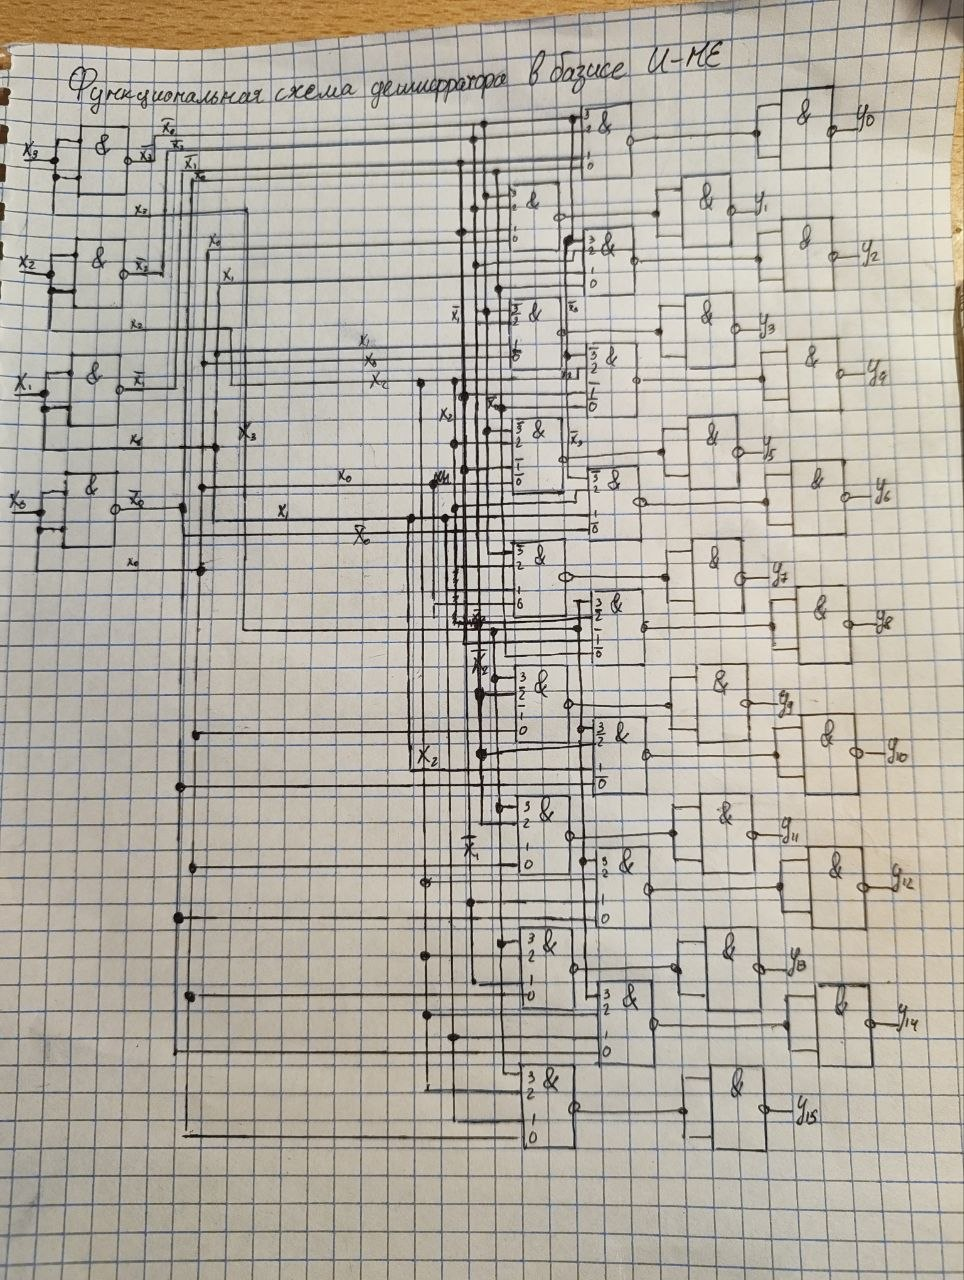
\includegraphics[width=0.85\textwidth,keepaspectratio]{pics/functional_diagram.jpg}
  \caption{Функциональная схема дешифратора в базисе <<И-НЕ>>}
\end{figure}

\newpage
\section{Синтез демультиплексора на основе дешифратора}
Демультиплексор (DMX) представляет собой коммутационное устройство, распределяющее цифровой сигнал с одного информационного входа $D$ на один из $N$ выходов в соответствии с приходящим адресным кодом. 

С точки зрения логической структуры, демультиплексор <<1 в 16>> полностью повторяет схему полного дешифратора <<4 в 16>>, у которого каждый конъюнктивный терм умножается на логическую переменную входных данных $D$.

Применение функционально полного базиса И-НЕ (штрих Шеффера) к структуре демультиплексора также требует введения двойного отрицания для сохранения активного высокого уровня на выбранном выходе. Логические уравнения выходов демультиплексора принимают следующий вид:

\begin{align*}
  y_0  &= \overline{\overline{D \cdot \overline{x}_3 \cdot \overline{x}_2 \cdot \overline{x}_1 \cdot \overline{x}_0}} & 
  y_8  &= \overline{\overline{D \cdot x_3 \cdot \overline{x}_2 \cdot \overline{x}_1 \cdot \overline{x}_0}} \\
  y_1  &= \overline{\overline{D \cdot \overline{x}_3 \cdot \overline{x}_2 \cdot \overline{x}_1 \cdot x_0}} & 
  y_9  &= \overline{\overline{D \cdot x_3 \cdot \overline{x}_2 \cdot \overline{x}_1 \cdot x_0}} \\
  y_2  &= \overline{\overline{D \cdot \overline{x}_3 \cdot \overline{x}_2 \cdot x_1 \cdot \overline{x}_0}} & 
  y_{10} &= \overline{\overline{D \cdot x_3 \cdot \overline{x}_2 \cdot x_1 \cdot \overline{x}_0}} \\
  y_3  &= \overline{\overline{D \cdot \overline{x}_3 \cdot \overline{x}_2 \cdot x_1 \cdot x_0}} & 
  y_{11} &= \overline{\overline{D \cdot x_3 \cdot \overline{x}_2 \cdot x_1 \cdot x_0}} \\
  y_4  &= \overline{\overline{D \cdot \overline{x}_3 \cdot x_2 \cdot \overline{x}_1 \cdot \overline{x}_0}} & 
  y_{12} &= \overline{\overline{D \cdot x_3 \cdot x_2 \cdot \overline{x}_1 \cdot \overline{x}_0}} \\
  y_5  &= \overline{\overline{D \cdot \overline{x}_3 \cdot x_2 \cdot \overline{x}_1 \cdot x_0}} & 
  y_{13} &= \overline{\overline{D \cdot x_3 \cdot x_2 \cdot \overline{x}_1 \cdot x_0}} \\
  y_6  &= \overline{\overline{D \cdot \overline{x}_3 \cdot x_2 \cdot x_1 \cdot \overline{x}_0}} & 
  y_{14} &= \overline{\overline{D \cdot x_3 \cdot x_2 \cdot x_1 \cdot \overline{x}_0}} \\
  y_7  &= \overline{\overline{D \cdot \overline{x}_3 \cdot x_2 \cdot x_1 \cdot x_0}} & 
  y_{15} &= \overline{\overline{D \cdot x_3 \cdot x_2 \cdot x_1 \cdot x_0}}
\end{align*}

Функции демультиплексора также не подлежат минимизации, так как информационный сигнал должен транслироваться на выходы без логических искажений, а адресные переменные выполняют функцию селекторов каналов.

\section{Модернизация функциональной схемы}
Для аппаратного перевода схемы дешифратора в режим демультиплексора матричная шинная структура дополняется одной вертикальной входной шиной данных $D$. 

Поскольку исходные элементы логического умножения адреса имели 4 входа, добавление переменной $D$ расширяет разрядность элементов первого каскада. Схема модернизируется путем замены 16 элементов <<4И-НЕ>> на элементы <<5И-НЕ>>. На свободный пятый вход каждого элемента параллельно заводится шина данных $D$. Оконечные двухвходовые инверторы И-НЕ остаются без изменений.

\begin{figure}[H]
  \centering
  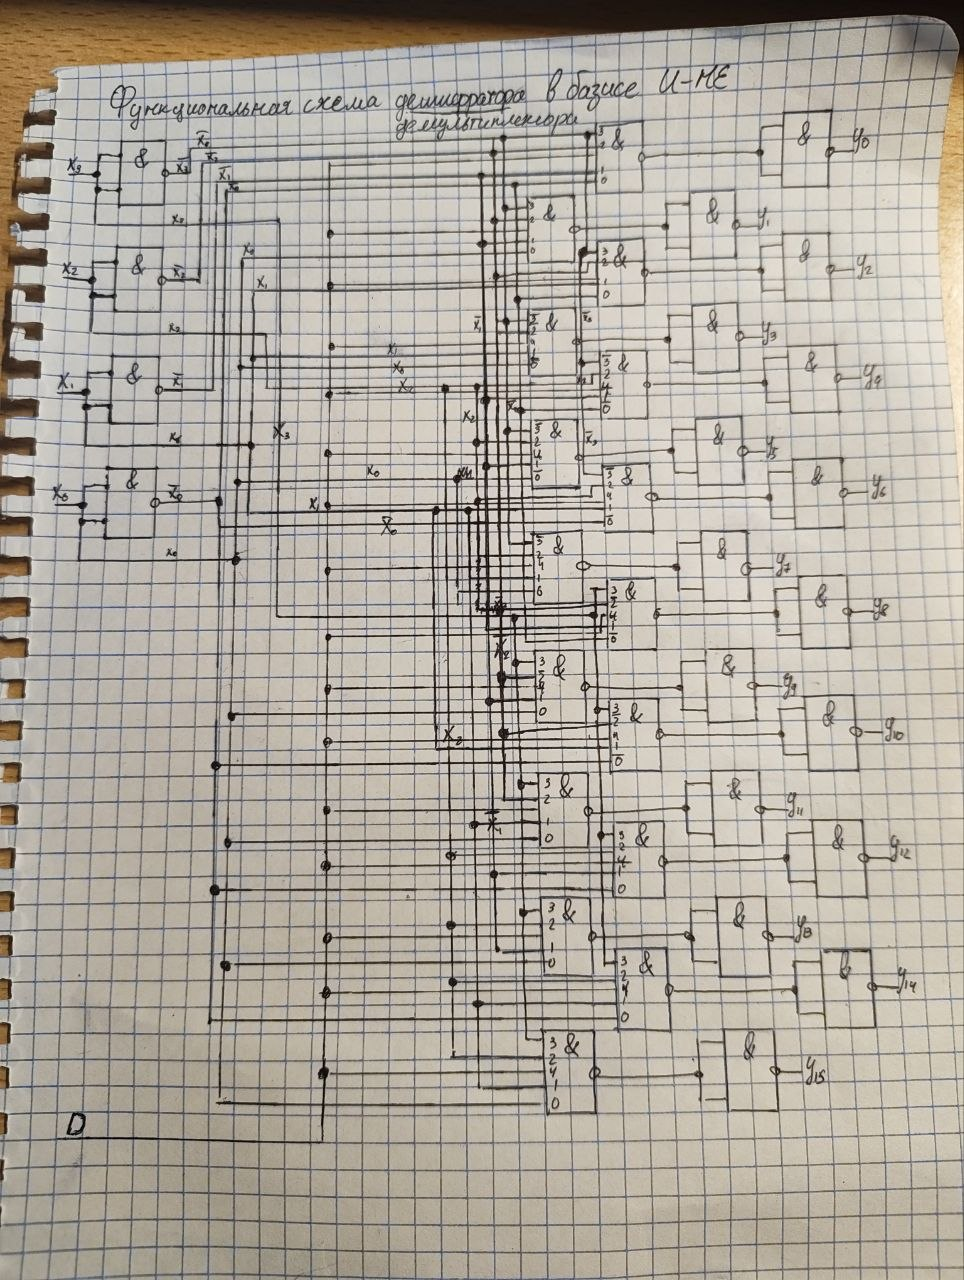
\includegraphics[width=0.85\textwidth]{pics/demux_functional.jpg}
  \caption{Функциональная схема демультиплексора в базисе <<И-НЕ>>}
\end{figure}

\section*{Вывод}
В ходе выполнения контрольной работы были изучены принципы построения многовыходных комбинационных цифровых устройств. На примере полного дешифратора <<4 в 16>> и демультиплексора <<1 в 16>> в базисе Шеффера была продемонстрирована их глубокая структурная взаимосвязь: схема дешифратора является базисом для демультиплексора, преобразуясь в него путем расширения логических элементов первого каскада дополнительным информационным входом $D$. Проектирование в едином логическом базисе И-НЕ показало высокую эффективность матричного метода компоновки сложных логических схем.

\end{document}